\section{Evaluation}
\label{sec:results}

% \subsection{Validation of eBPF processor}

% \begin{figure}[bth]
% \centering
% %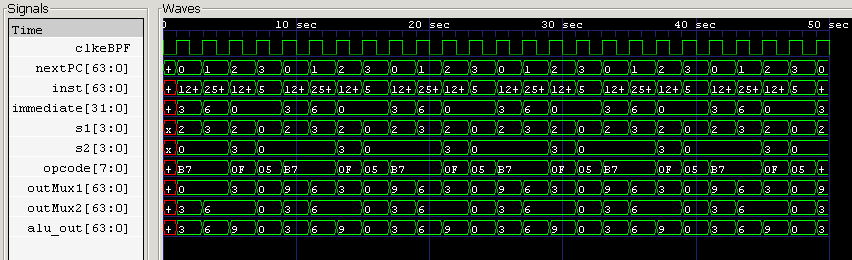
\includegraphics[width=1.\textwidth]{figures/07_fig02.png}
% 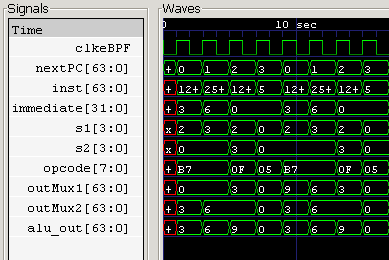
\includegraphics[width=1.\linewidth]{figures/07_fig02half.png}
% \caption{eBPF processor waveform instruction tests.}
% \label{fig:07_fig02}
% \end{figure}


% Firstly, for validation of the eBPF processor, we used the Altera Cyclone IV EP4CE115 platform. This FPGA has 114,480 logic cells, 50 MHz clock cycle and a set of memories (EEPROM, SRAM, Flash) with a storage capacity of 8 to 128 MB. We use the Altera platform with the aim of detecting and also correcting errors quickly before integrating the processor into the NetFPGA data path.


% % \begin{figure}[H]
% % \centering
% % \includegraphics[width=1.\textwidth]{imagens/06_fig10.png}
% % \caption{Forma de onda  processador eBPF.}
% % \label{fig:06_fig10}
% % \end{figure}




% Figure~\ref{fig:07_fig02} presents the generated waveform of the execution of an assembly program containing the following instructions: mov64, add, and ja (jump absolute). The first instruction to execute is an immediate mov64. In this instruction, register r2 receives the immediate value 3. The second instruction is also an immediate mov64. The register r3 receives the value 6. In the third instruction, the sum operation between r2 and r3 is executed. Both operations use the register file to read and write to the respective registers. Register r2, at the end of the sum operation, has value 9 and stores it in the register file. The last instruction is a jump to the beginning of the code, the program counter goes to zero, initializing its operations. The last line in the Figure (alu\_out), represents the output of the ALU according to each instruction.


% With the exception of the call instruction, as explained earlier, the eBPF processor has been synthesized and tested for all eBPF instructions on an Intel Altera platform. Then, the same processor was synthesized in Xilinx Vertex-II Pro 50 FPGA. Xilinx software synthesized all instructions except multiplication, division, and remainder instructions. In practice, these instructions are not widely used on a switch. In addition, these instructions with the power of 2 can be executed with the operations shift left, shift right, and logical operator and, respectively. We believe that a newer version of NetFPGA can accept the synthesis of these instructions. The project with the inclusion of these instructions, described in Verilog, is correctly synthesized in the Intel Altera FPGA development environment.

%Na figura~\ref{fig:06_fig11}

Here, we present the experimental evaluation of eBPFlow. 
% To understand its capabilities and limits we performed several experiments on a controlled environment (\textsection\ref{sec:experiments}) with several use cases (\textsection\ref{sec:use-cases}). We validated eBPFlow's ability to perform zero downtime program switch (\textsection\ref{sec:downtime}), measured throughput, and latency for each NF (\textsection\ref{sec:performance}) and also its power consumption (\textsection\ref{sec:power}).  

\subsection{Test environment} 
\label{sec:experiments}

% \begin{figure}[ht]
% \centering
% 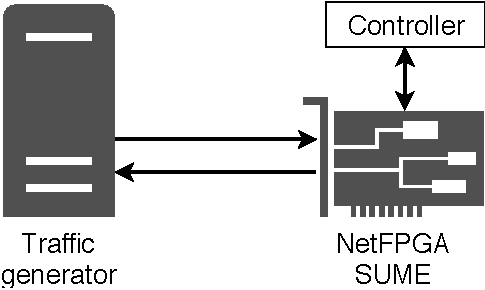
\includegraphics[width=0.7\columnwidth]{figures/test-topology-ebpflow.pdf}
% \caption{Topology of the experiments.}
% \label{fig:07_fig03}
% \end{figure}

% Figure~\ref{fig:07_fig03} presents the topology used to run the experiments, 

The test topology used during tests consisted on one NetFPGA SUME, one server running \textit{pktgen-DPDK}~\cite{Pktgen2016} acting as a traffic generator, and a custom controller used to interact with the eBPFlow processor. The server was equipped with a Netronome Agilio CX SmartNIC with two 10 Gbps interfaces. Each 10 GbE port is connected directly to each of two active NetFPGA ports, sending network traffic at line rate, following the same configuration as~\cite{FlowBlaze2019}. Thus, the NetFPGA can receive and send 10~Gbps simultaneously. Both the traffic generation server and the server holding the NetFPGA were powered by i7-7700 \@ 3.60~GHz processors with 8 cores and 8~GB of RAM.


% We developed C language applications. The code is compiled with LLVM 3.9 for the eBPF big endian platform. The LLVM compiler generates an executable in the executable and link format (ELF). The objcopy tool extracts the instruction set from the .text segment of the elf file.
% The controller installs this segment into eBPFlow.

\subsection{Use cases}
\label{sec:use-cases}

We implemented several network programming code (Table~\ref{tbl:example-sizes}) to stress test the generality of eBPFlow's expressive abstraction as a network packet processing core.
For each network function (NF), we present the number of eBPF instructions and the number of C code lines. 
These NFs were chosen because they are used as benchmark evaluation in the network literature~\cite{Panda:2016,Sun:2017:NEN:3098822.3098826}.
%The applications are ordered in Table~\ref{tbl:example-sizes} according to the number of instructions}, where. 
% $LU$ indicates programs compiled with Loop Unrolling (LU) enabled. From Figure~\ref{fig:Language}, the $LU$ enabled programs are classified as eBPF-verifier. These programs require more instructions since the loop has to be unrolled. 
The description of each NF is as follows:

\begin{table}[t]
\centering
\caption{eBPF programs used during experiments.}
\label{tbl:example-sizes}
\resizebox{\linewidth}{!}{%
\begin{tabular}{|l|c|c|}
\hline
\textbf{Network programs} & \textbf{\#Instructions} & \textbf{\#LoC in C}\\  \hline
Return                & 4                         & 8\\ \hline
Wire             & 5                         & 8\\ \hline
%wire                  & 7                       &\\ \hline
Learning Switch       & 27                       & 35\\ \hline
IPv4 Router           & 30                       & 35\\ \hline
DDoS Mitigation       & 35                       & 82\\ \hline
%l4lb                  & 155                     & \\ \hline
NAT                   & 182                      & 229\\ \hline
% ChaCha8  (w/o LU) &     575            & 356\\ \hline
% ChaCha20 (w/o LU) &     575          & 356\\ \hline
% ChaCha8  (w/ LU)  &     1,543        & 356\\ \hline
% ChaCha20 (w/ LU)  &     3,965        & 356\\ \hline
\end{tabular}}
\end{table}

\textbf{Return:} is the simplest application possible. It forwards packets to a fixed port and serves as a performance baseline. 

\textbf{Wire:} acts as wire connecting adjacent ports in pairs of two. It performs an XOR operation between the input port value and 1, which flips the least significant bit. This value sets the packet's output port.

\textbf{L2 Learning Switch} (\texttt{L2LS}): a functional learning switch capable of forwarding Ethernet frames based on values learned on demand and stored on the CAM.

% The advantage of a protocol-independent switch is that it only needs to parse the frame header fields for the protocols defined by the programmer. In this example, the parser only needs to parse Ethernet headers, while a protocol-dependent switch would process other frame or packet header fields. CAM (exact-match) lookup table stores the Ethernet MAC address and the input port. 
% For each input frame, if the source address is unicast, the code can self-populate the lookup table by updating it. This second advantage can reduce network traffic, latency, and CPU controller overhead. Using the destination MAC, the output port is searched. If there is an entry, then the packet is forwarded otherwise there are two options. It can be flooded or sent to the controller. In this experiment, we opted to flood.

\textbf{IPv4 Router} (\texttt{IP4R}): routes packets using the NetFPGA's TCAM module, effectively speeding up costly longest prefix matching operations. 

\textbf{DDoS Mitigation:} mitigates DDoS attacks by analyzing and dropping potentially dangerous packets on demand~\cite{Bertin2017}.

\textbf{Network Address Translation} (\texttt{NAT}): modifies packets and stores flow state. Several CAM entries were used to store flow information to translate inbound and outbound packets.

%Não tenho esssa informação. 
%The code is installed through the NetFPGA register interface. The time to read or write one register in this interface is 500 us. Each eBPF instruction (64 bits) utilizes two registers (32 bits). To start the code installation, it requires 2 write operations.
%Thus, the time to install a code is given by:\\Time to install code $=$ (number of instructions+2) $* 500 us * 2.$ 

% In the last experiment, eBPFlow starts as IPv4 router. During runtime, we install the learning switch. This experiment validates the system by showing that the switch executes these instructions for each received packet, allowing a data plane with dynamic parse, matching, and actions at run time with zero downtime.

% \textbf{ChaCha:} 
% ChaCha20~\cite{rfc8439} network function is a
% stream cipher used in Transport Layer Security (TLS) by Google for symmetric
% encryption~\cite{google-chacha}.
% ChaCha20 cannot be implemented in the P4 switch.
% The number after ChaCha indicates how many rounds to apply the cipher over the data.
% We tried to implement it on the Netronome Agilio CX 1x40 Gbps SmartNIC but it can only support up to eight rounds. Netronome expressiveness can be categorized as eBPF-verifier. It requires the verifier and loop unrolling, which increases the number of instructions and thus does not fit in the smartNIC memory instruction.
% But, \system is able to execute ChaCha20.


\subsection{Zero downtime}
\label{sec:downtime}

\begin{figure}[th]
\centering
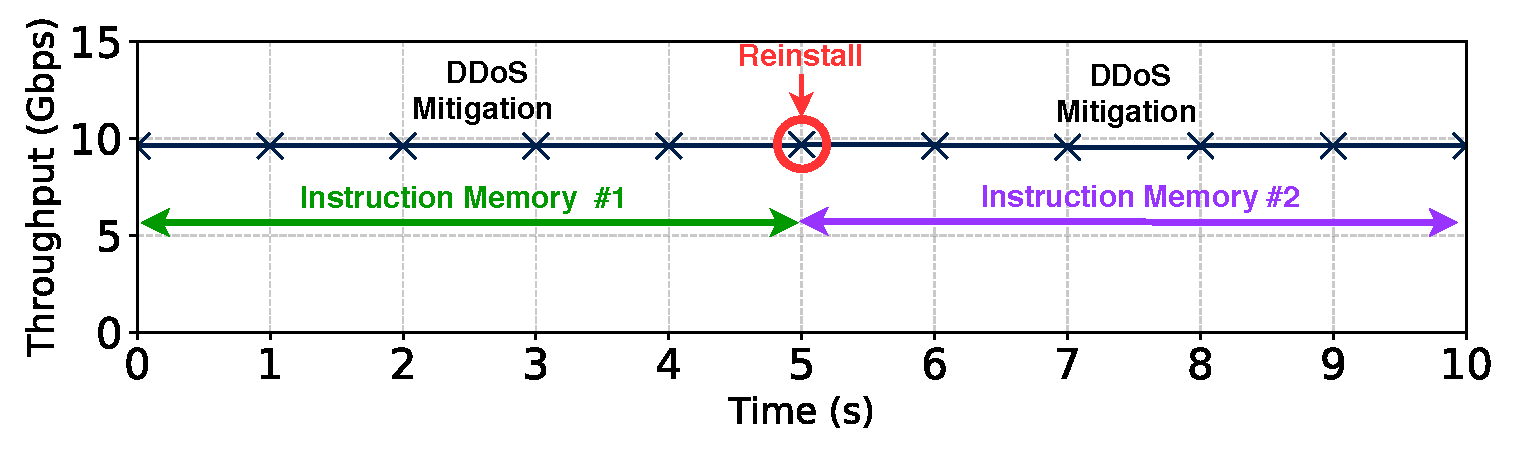
\includegraphics[width=1.\linewidth]{figures/zero_downtime.pdf}\caption{Zero downtime using DDoS Mitigation NF.}
\label{fig:zerodowntime}
\end{figure}



We evaluated the system capability to modify parsing, matching, and actions at run time with zero downtime using the DBS instruction memory. Figure~\ref{fig:zerodowntime} shows the throughput (in Gbps) before, during, and after loading a new eBPF program. We send a constant rate of 512-byte packets at 10 Gbps and switch the processor's program during runtime. Before the experiment begins, the processor is loaded with the DDoS mitigation program on one of the instruction memories. At $t=5$ s, a different DDoS mitigation program is loaded, representing an update on the mitigation policy. 
%A special register stores the ID of the current instruction memory in use and, whose value is shown in Figure~\ref{fig:zerodowntime}. After the switch the new program's instructions are successfully stored on the second instruction memory and.
No packets are dropped in this process, showing zero downtime during loading.
% To ensure the new was installed at a different instruction memory, a special register was added to store the ID of the current instruction memory in use. Figure~\ref{fig:zerodowntime} demonstrates that the change between eBPF programs no cause packets loss after the installation of another eBPF program.
% Thus, the system can dynamic load new NFs.

\subsection{Program scheduling}

In this experiment, we evaluate the functionality of eBPFlow's Serverless Computing platform. Two different allocation requests are sent from the controller to the scheduler running on the server that powers the NetFPGA. Both requests consist of a Return-like program ($P1$ and $P2$) to be run for 5 seconds each. The programs just forward the packet to output ports 0 and 1, respectively. This time, we used an extra Intel X710 NIC to generate and receive traffic from the NetFPGA (total of 4 interfaces), and traffic was generated from port 3, as illustrated by Figure~\ref{fig:request}.
 
\begin{figure}[H]
\centering
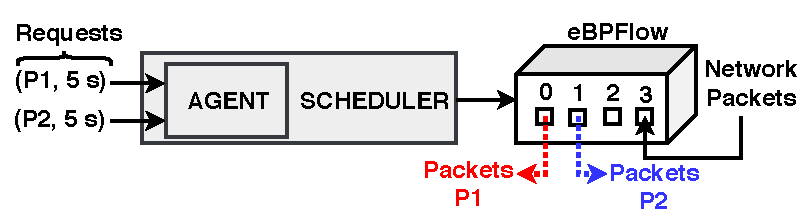
\includegraphics[width=1.0\columnwidth]{figures/request.pdf}
\caption{Experiment topology.}
\label{fig:request}
\end{figure}

The first program to be scheduled is $P1$, which forwards traffic to output port. At $t=~5$, its scheduled time expires and the scheduler loads $P2$. Due to DBS, the programs are switched only when the new program is fully loaded to the idle instruction memory, and the switch occurs atomically (\S~\ref{sec:downtime}). Figure~\ref{fig:jobsched} shows the throughput received by ports 0 and 1 on the traffic generator, directly connected to the NetFPGA. We modified \textit{pktgen-DPDK}'s source code to reduce the minimum sampling period from $1 s$ to $1 ms$ and collect the amount of packets received by each port every millisecond. The apparent transition of $2$ ms shown in Figure~\ref{fig:jobsched} is caused by low sampling rate. The switch happens at $4.999$ s, but after the sample taken. The next sample will account for the packets sent during that interval, leading to a transition state at $t=5$, in which both ports seem to be receiving packets. Nonetheless, this shows the scheduler is capable of switching programs dynamically on-the-fly according to the requested allocation.

%\begin{figure}[th]
%\centering
%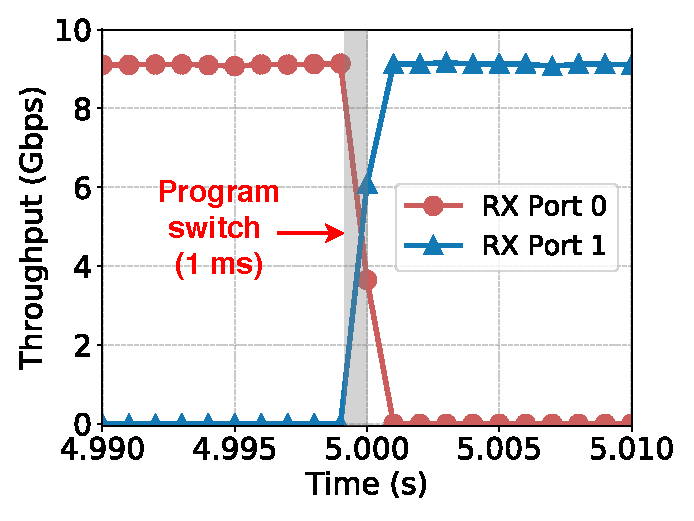
\includegraphics[width=\linewidth]{figures/job-sched.pdf}
%\caption{Time to transition between programs.}
%\label{fig:jobsched}
%\end{figure}

\subsection{Throughput}
\label{secsec:throughput}

Figures~\ref{fig:throughput64} and~\ref{fig:throughput128} summarize the measured packet processing rates of minimum- (64 bytes) and 128-sized packets, respectively, for each NF for one interface (as in~\cite{FlowBlaze2019}). The optimized version refers to the DM\_FIFO component that allows zero copy and processing the packet before receiving the entire packet. The optimized versions of Wire and Return programs achieve the highest rate in both cases, which is expected due to their simplicity and low number of instructions. As we increase the packet size, the packet processing overhead decreases, and the throughput increases, which was also expected. The reduced throughput achieved by the other examples is caused by lookups and updates on the TCAM/CAM, which takes several cycles and thus causes. This is even clearer for the NAT example, that beside having much more instructions than the other NFs, also performs several writes to the CAM, each taking 16 cycles each and stalling the processor.

\begin{figure*}[th]
  \centering
   \begin{minipage}[b]{0.3\textwidth} % Here
     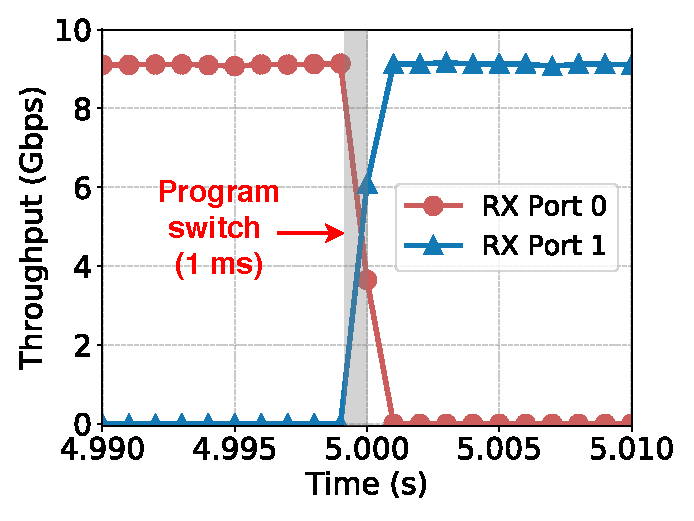
\includegraphics[width=1.\linewidth]{figures/job-sched.pdf}
     \caption{Program scheduling.}
     \label{fig:jobsched}
   \end{minipage}
    \hspace{0.2cm}
  \begin{minipage}[b]{0.3\textwidth}
    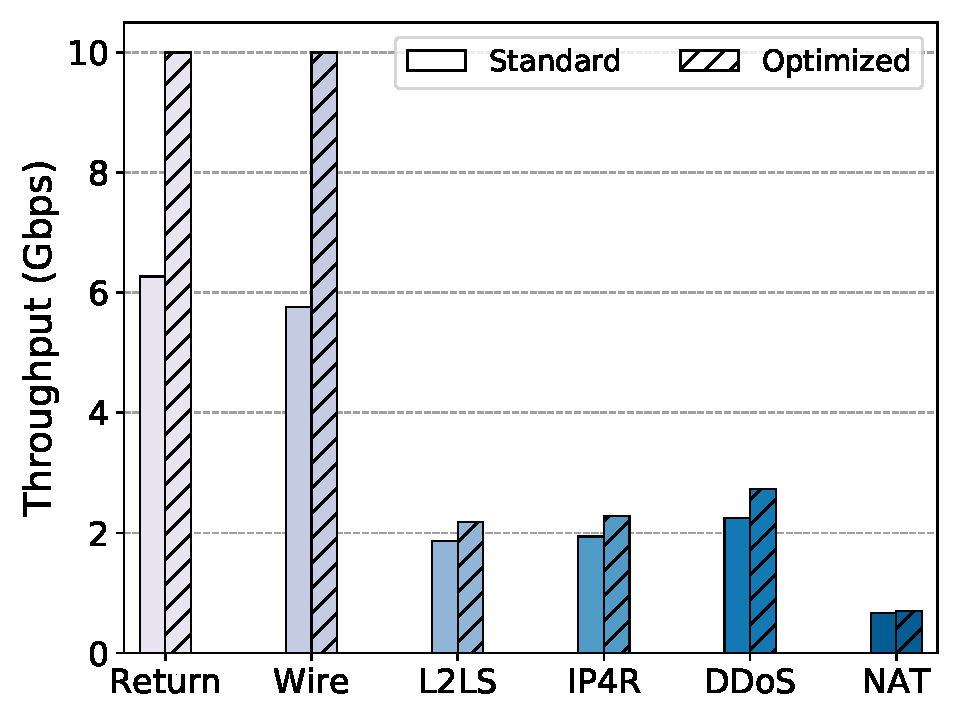
\includegraphics[width=.98\textwidth]{figures/throughput_gbps_64B.pdf}
    \caption{Throughput (64 Bytes).}
    \label{fig:throughput64}
  \end{minipage}
  \hspace{0.2cm}
  \begin{minipage}[b]{0.3\textwidth}
    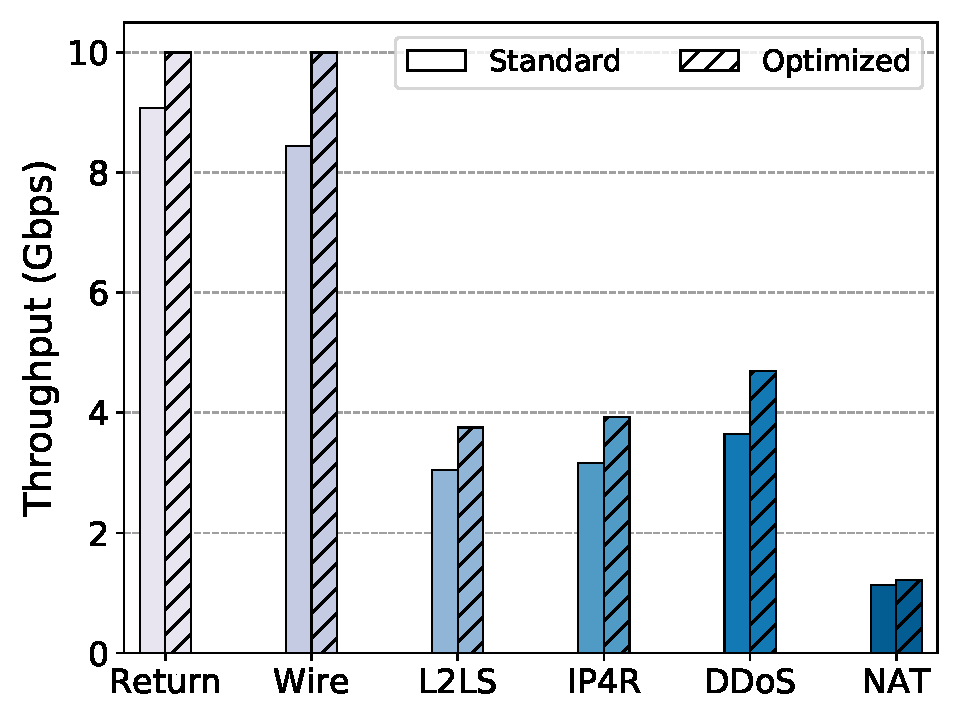
\includegraphics[width=.98\textwidth]{figures/throughput_gbps_128B.pdf}
    \caption{Throughput (128 Bytes).}
    \label{fig:throughput128}
  \end{minipage}
  \hspace{0.2cm}
  \begin{minipage}[b]{0.3\textwidth}
    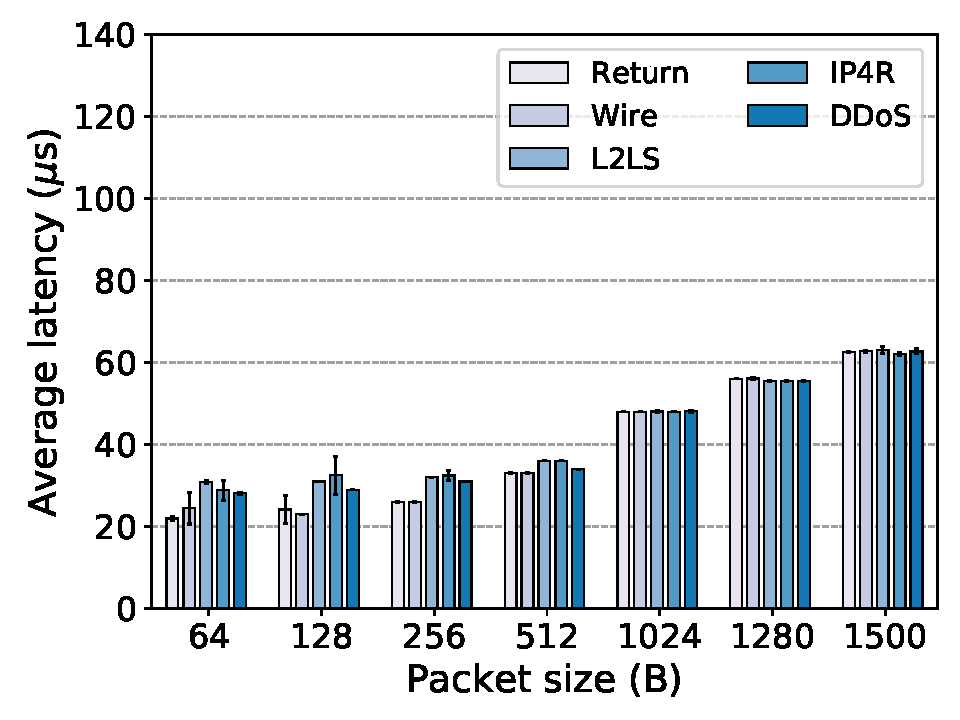
\includegraphics[width=1.\textwidth]{figures/latency.pdf}
    %\caption{Average latency per packet sizes and NFs.}
    \caption{Average latency.}
    \label{fig:latency}
  \end{minipage}
  \hspace{0.2cm}
  \begin{minipage}[b]{0.3\textwidth}
    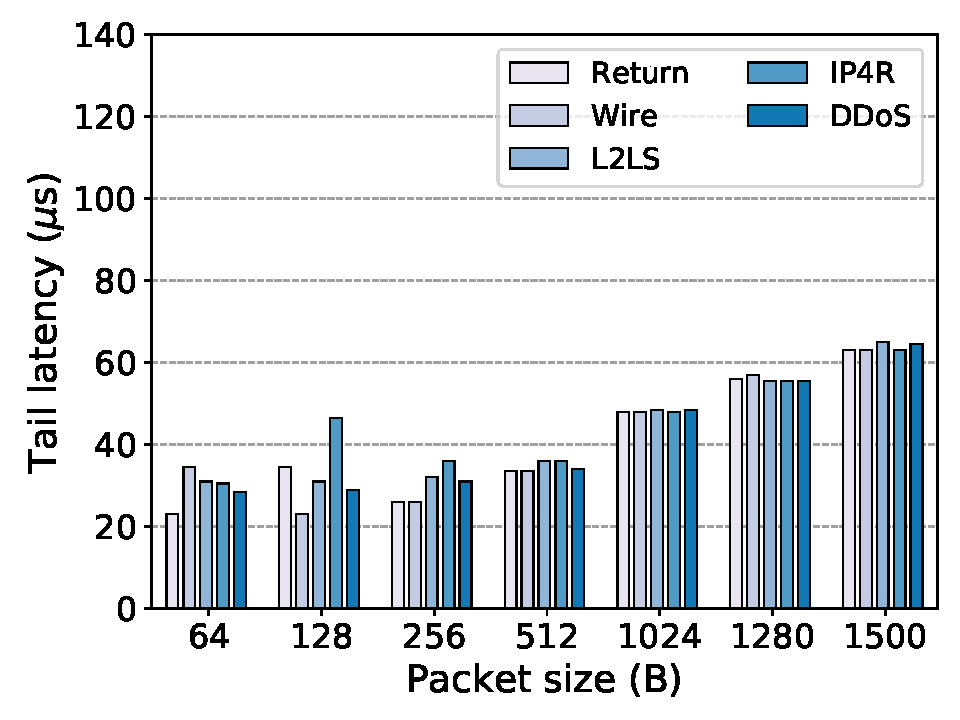
\includegraphics[width=1.\textwidth]{figures/taillatency.pdf}
    %\caption{Tail latency for different packet sizes and NFs.}
    \caption{99th-percentile latency.}
   \label{fig:taillatency}
 \end{minipage}
 \hspace{0.2cm}
 \begin{minipage}[b]{0.3\textwidth} % Here 
   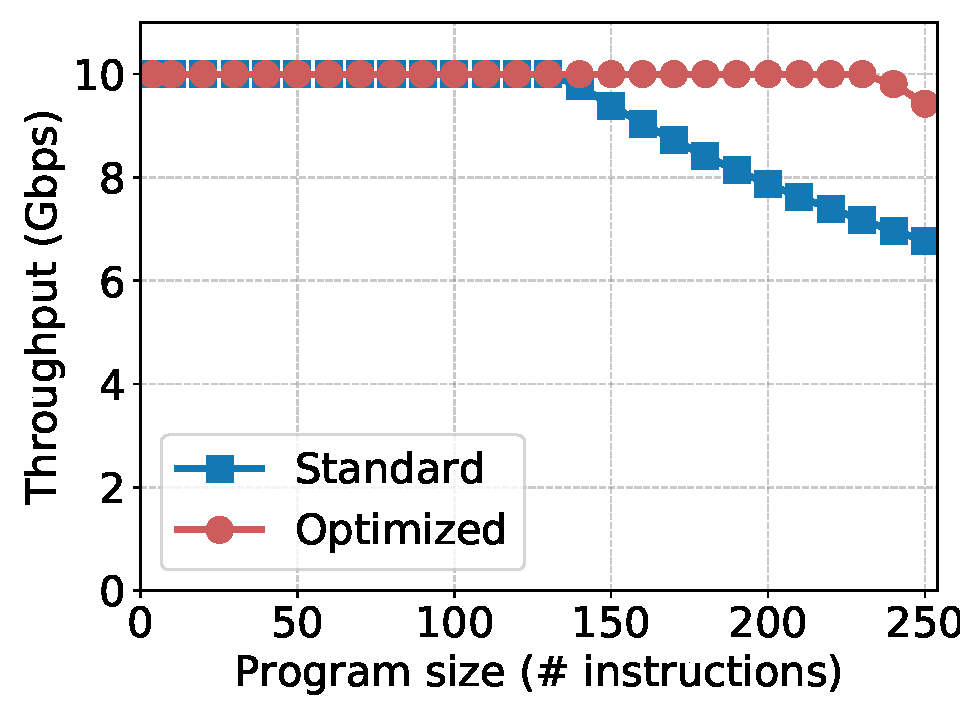
\includegraphics[width=.98\textwidth]{figures/throughput_prog_size.pdf}
   \caption{Impact of program size.}
   \label{fig:programsize}
 \end{minipage}

\end{figure*}

%Figure~\ref{fig:throughput64} summarizes the measured packet processing rates of minimum-sized (64 bytes) packets with many NFs in Mpps for one interface (as in~\cite{FlowBlaze2019}).
% As discussed in Figure~\ref{fig:Comparison}, there is a trade-off between flexibility and performance.
% We have quantified this trade-off. Figure~\ref{fig:throughput1500} shows eBPFlow's achieved throughput when processing packets of 1500 bytes. 
%Wire and Return programs achieve the highest rate in both cases for their simplicity and low number of instructions.
% Figure~\ref{fig:throughput1500} shows that almost all examples are capable of maximum line rate with 1500 B packets, NAT being an exception with at approximately 8 Gbps, which performs 3 CAM lookups, thus being more computationally expensive than the other examples.

% This decrease in performance is caused by the cost of packet copies done inside the packet processing pipeline. It becomes specially acute for small packets (64 B) because of the very short time between packet arrivals, which leaves little slack for the processor to finish processing the previous packet. 

% \begin{figure}[th]
% \centering
% 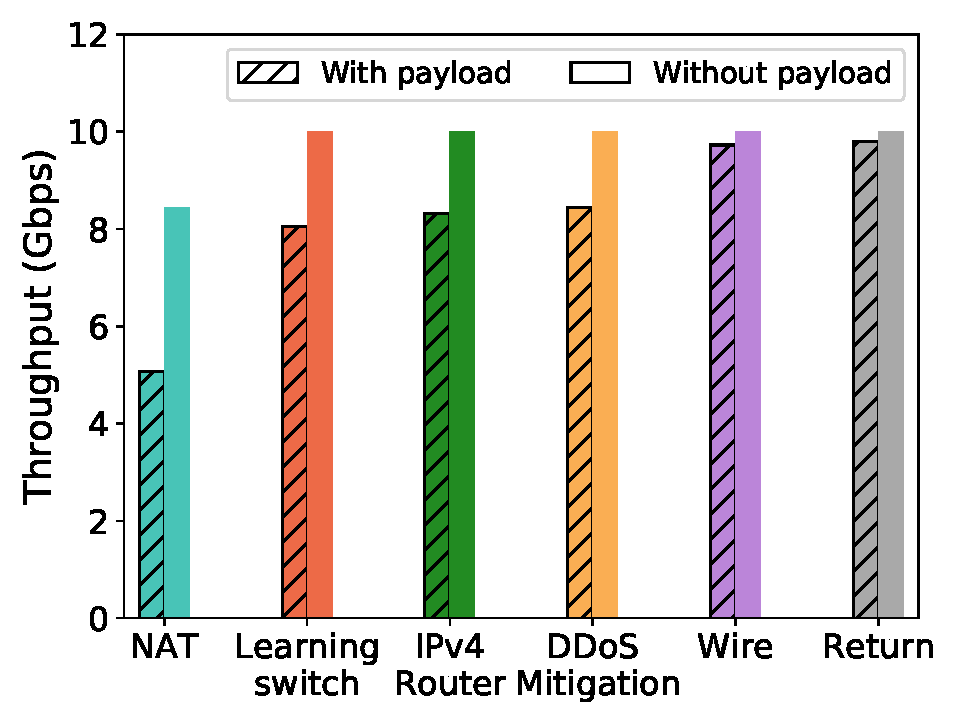
\includegraphics[width=.85\columnwidth]{figures/payload-1500B.pdf}
% \caption{Throughput with and without enabling payload processing.}
% \label{fig:payload-1500B}
% \end{figure}

% \begin{figure}[th]
% \centering
% 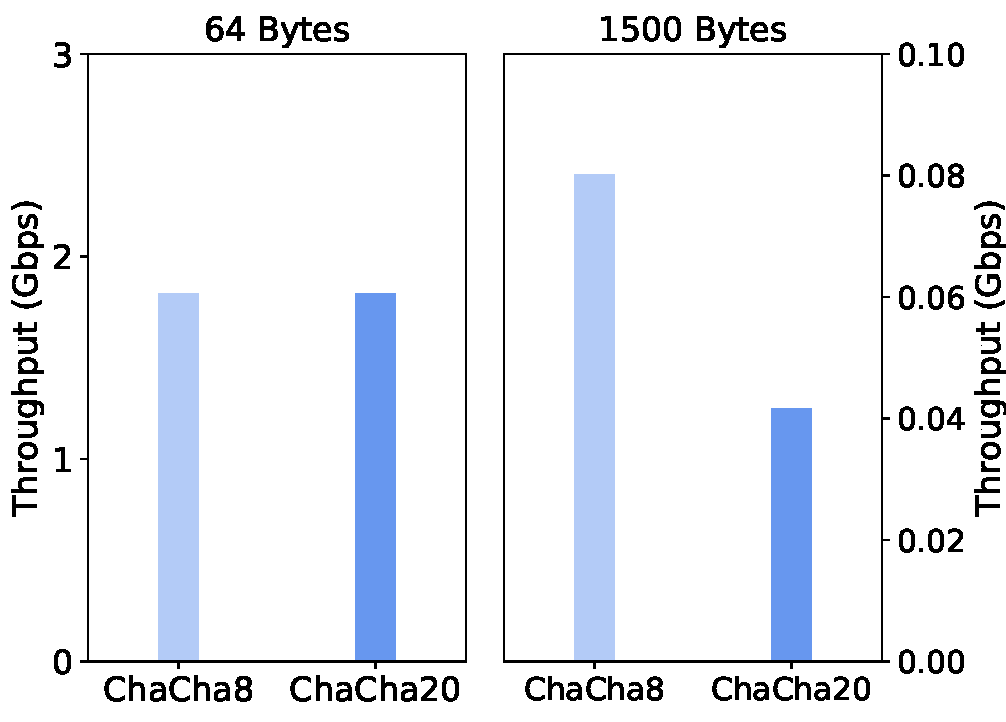
\includegraphics[width=.8\linewidth]{figures/throughput_chacha.pdf}
% \caption{Throughput for ChaCha8 and ChaCha20 examples}
% \label{fig:chacha}
% \end{figure}

% As describe in \textsection\ref{secsec:actions}, the controller can decides if the device should process the entire packet or just the headers (like dRMT~\cite{chole2017drmt} does). 
% %The controller sends a signal that enables or disables the processing of the packet's payload on eBPFlow's.
% This optimization allows processing the payload only for NFs that need it (e.g., ChaCha8 and ChaCha20).
% To demonstrate the difference in performance obtained with this optimization, the same set of experiment was executed (1500 B packets at 10 Gbps) in two different scenarios: with and without payload processing. Figure~\ref{fig:payload-1500B} presents the throughput in Gbps for each of the example NFs. 
% Hatched bars represent programs executed with payload signal enabled, while plain bars indicate processing without the payload. 
% %Packets of 1500 bytes were used in this experiment since they represent the standard MTU used by most networks. 
% When the payload signal is enabled, all NFs decreases their throughput since there is an overhead to transfer the payload.
% %To improve eBPFlow's throughput performance even further it's necessary add support for zero copy processing.



% Figure~\ref{fig:chacha} presents the results for ChaCha8 and ChaCha20 with packet sizes of 64 and 1500 bytes. These NFs present better performance for minimum-sized packets since they process the payload.
% %On the other hand, processing bigger packets come at a high cost as shown by the low throughput achieved with 1500-byte packets. 
% Although at a low rate, eBPFlow is the only platform capable of running ChaCha20, whereas other platforms like P4, Netronome eBPF, FlowBlaze cannot.

\subsection{Latency}

In addition to the throughput, we also measured the average and tail latencies for each NF (Figures~\ref{fig:latency} and~\ref{fig:taillatency}) using \textit{pktgen-DPDK}, with 1 $\mu s$ precision.
% In addition to throughput measurements, \textit{pktgen}'s builtin support for latency measurement was used to evaluate the average latency for each use case, which is shown in Figure~\ref{fig:latency}. All measurements were taken with at a rate of 1 Gbps. 
As expected, latency increased with the number of instructions (see Table \ref{tbl:example-sizes}), since the processor will take more time to run the entire program. The bars on Figure~\ref{fig:latency} represent the standard deviation, which was close to zero in most cases. This demonstrates that there is little change on the processing time between same-sized packets for a single NF, consequently leading to reduced jitter. Similarly, the tail latency is close to the average value in almost all cases.
% Measurements for ChaCha8 and Chacha20 were not included due to an incompatibility with \textit{pktgen}. The tool uses the packet's payload to store metadata used to estimate latency. Since these two applications encrypt the payload, \textit{pktgen} was not able to retrieve the metadata at the RX port.

% The latency profile shown by the NAT is due to a combination of queuing, processing delays and accessing CAM. For small packet sizes the NAT's processing delay causes eBPFlow's input queues to grow, since the packet arrival rate is high. As the packet size increases, this rate gets smaller, reducing the queuing effect. However, starting at 1024 B, the effect of moving payload inside the processing pipeline starts to rule the total, and the average latency grows again.
% %This behavior is expected since the actual time to process the instructions is the same for all packets sizes as the NAT only touches a few fields in the packet headers, however queuing and copying delays have different influences on packet sizes.

\subsection{Program size impact}

To understand the impact of program size on the observed performance, we created $26$ synthetic programs consisting of a varying number of \textit{mov} instructions and a final \textit{exit} instruction. Besides the smallest value (4 instructions), we varied program sizes from $10$ to $250$, increasing $10$ instructions at a time. The traffic generated consisted of 1500-byte packets at 10 Gbps. Figure~\ref{fig:programsize} presents the throughput obtained for each program, considering both eBPFlow versions (Standard and Optimized). There are two main takeaways from these results. First, the DM\_FIFO optimization allowed achieving line rate for larger programs, due to the reduced number of packet copies needed when compared to the standard version. Second, eBPFlow is potentially capable of much higher rates than the ones observed for the example programs. The results in \S~\ref{secsec:throughput} are affected by TCAM/CAM lookups/writes, which have greater cost than simple \textit{mov} instructions that execute in a single cycle. As future work, we plan to mix such high-cost instructions into the workload to further analyze their impact.

%\begin{figure}[H]
%\centering
%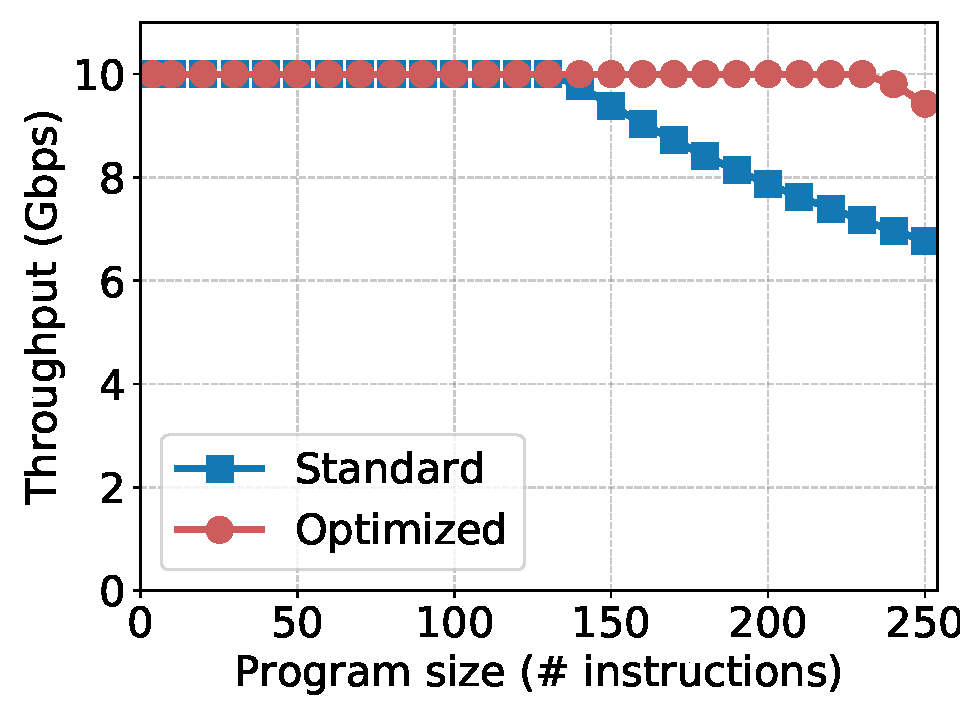
\includegraphics[width=\linewidth]{figures/throughput_prog_size.pdf}
%\caption{Impact on throughput caused by program size growth.}
%\caption{Impact of program size on overall throughput.}
%\label{fig:programsize}
%\end{figure}



\subsection{Power}
\label{sec:power}

%When idle, the NetFPGA consumes 16 W. When eBPFlow is loaded, the power consumption is 22 W independent of the packet rate or what programming is running. On the other hand, an idle CPU already consumes 85 W. Thus, eBPFlow saves power in comparison to software packet processing.

Table~\ref{tab:powerconsumption} presents the power consumption of some packet processing devices. When idle, the NetFPGA consumes 16 W. When eBPFlow is synthesized, the power consumption is 22 W regardless of the packet rate or what programming is running. 
%Netronome's SmartNIC consumes between 20 W and 40 W when active. 
eBPFlow has lowest power consumption per-interface (5.5 W).
%An idle CPU already consumes 85 W. 
An x86 server spends 55x more power than eBPFlow.
Thus, eBPFlow saves power in comparison to other packet processing devices.

%P4 switches (i.e., P4 Wedge 100BF-32X) spent 20 times more energy than eBPFlow. x86 server is the equipment with greater consumption in packet processing.


%\textcolor{red}{The Power of SmartNICs reference} \cite{powersmartnics}. 

\begin{table}[h] %tb
\centering
\caption{Devices power consumption comparison.}
\label{tab:powerconsumption}
\begin{tabular}{|c|c|}
\hline \textbf{Device} & \textbf{Power consumption} \\ \hline
NetFPGA SUME (idle)  & 16 W \\ \hline
eBPFlow  & 22 W \\ \hline
Netronome's SmartNIC~\cite{NetronomePC} & up to 40 W \\ \hline
%CPU (idle)  & 85 W \\ \hline
Intel Core i7-7700~\cite{i7i7700} & 65 W \\ \hline
P4 Wedge 100BF-32X~\cite{P4wedge} & 436 W \\ \hline
x86 server~\cite{x86serverPC} & 500 W to 1200 W \\ \hline
\end{tabular}
\end{table}


